% !TEX root = ../md2-user-handbook.tex
% !TeX spellcheck = en_GB
% !TeX program = xelatex

\lstset{language=Simple}

The current implementation of the \MD framework generates web-based apps for a framework called map.apps, which is mainly based on JavaScript. Code generation of Android and iOS apps are also targeted, but not fully implemented yet.

The generated code for \mapapps can be subdivided into three parts: static \mapapps code, dynamically generated \mapapps code and a backend. The static \mapapps code contains the part of the code which does not depend on the models created in the \MD DSL. Since it is static, it does not need to be generated, but is required for the overall functionality of the generated apps. The dynamically generated part is completely dependent on the model. The backend is implemented in Java and contains static as well as dynamic code. However, it is completely generated. The backend provides a server which offers functionality such as data storage and communication accross apps.

Each of these three parts of the code is described in detail in the following.

% start of section for static map.apps implementation

\subsection{Static \mapapps Implementation}

The static \mapapps code is split into several bundles, which are then used by the generated \mapapps code. These bundles are located at \lstinline!src/main/js/bundles! and are explained in the following subsections.

\subsubsection{Form controls}

The form controls are defined within the bundle \lstinline!md2_formcontrols!. It uses and extends the existing \mapapps bundle \lstinline|dataform| with additional form elements, which can be used in \MD. Each factory defined within the bundle of \MD, specifies how a JavaScript-object can be transformed to a data form widget. To define an own dataform or to understand the concepts of a dataform component the \href{http://developernetwork.conterra.de/documentation/31/developers/dataform}{\mapapps documentation} will be helpful.

\begin{description}
	\item[DateTimeBoxFactory] Defines a form control for the component \lstinline|DateTimeInput|, which is identified by the keyword \lstinline|datetimebox|. The widget shows a view element showing the time and the date of a \lstinline|datetime| value.
	\item[GridPanelFactory] Defines a form control for the component \lstinline|GridLayoutPane|, which is identified by the keywords \lstinline|md2gridpanel| and \lstinline|gridpanel|. The widget enables to structure multiple view elements in a grid.
	\item[ImageFactory] Defines a form control for the component \lstinline|Image|, which is identified by the keyword \lstinline|image|. The widget is able to display a static image within your app.
	\item[SpacerFactory] Defines a form control for the component \lstinline|Spacer|, which is identified by the keyword \lstinline|spacer|. A spacer defines some white space between some components or within the grid of a \lstinline|GridLayoutPane|.
	\item[StackContainerFactory] Defines a form control for the component \lstinline|AlternativesPane|, which is identified by the keyword \lstinline|stackcontainer|. This widget encapsulates the stack container within \href{http://dojotoolkit.org/reference-guide/1.10/dijit/layout/StackContainer.html}{\lstinline|dijit/ layout/StackContainer|}. It provides a view elements which has multiple views, but shows only one, similar to a book or a slide show. The user can navigate between them using specific keys. 
	\item[TextOutputFactory] Defines a form control for the component \lstinline|Label|, which is identified by the keyword \lstinline|textoutput|. This widget enables to display uneditable text.
	\item[TooltipFactory] Defines a form control for the component \lstinline|Tooltip|, which is identified by the keyword \lstinline|tooltipicon|. This widget offers a tooltip behind a question mark icon.
	\item[UploadImageOutputFactory] Defines a form control for the component \lstinline|UploadedImageOutput|, which is identified by the keyword \lstinline|uploadimageoutput|. The widget is able to display an image within your app, which is uploaded/specified by the user. 
\end{description}

Special dataform elements enable the use of uploaded files. The \lstinline|UploadedImageOutput| displays image which have been uploaded by an app's user using a \lstinline|FileUpload| input element. Given that both elements are mapped to an entity's attribute of type \lstinline|file|, these elements retrieve an image from, or store an image on the server, respectively. For this procedure, a specialised \lstinline|remoteConnection| needs to be defined by the modeller, thus defining the remote location of this service and a local path where this service is able to store files (\lstinline|fileUploadConnection|). Consequently, this remote connection can be different from every other remote connection used e.g.\ by content providers.

\begin{figure}[b!]
\centering % trim=l b r t
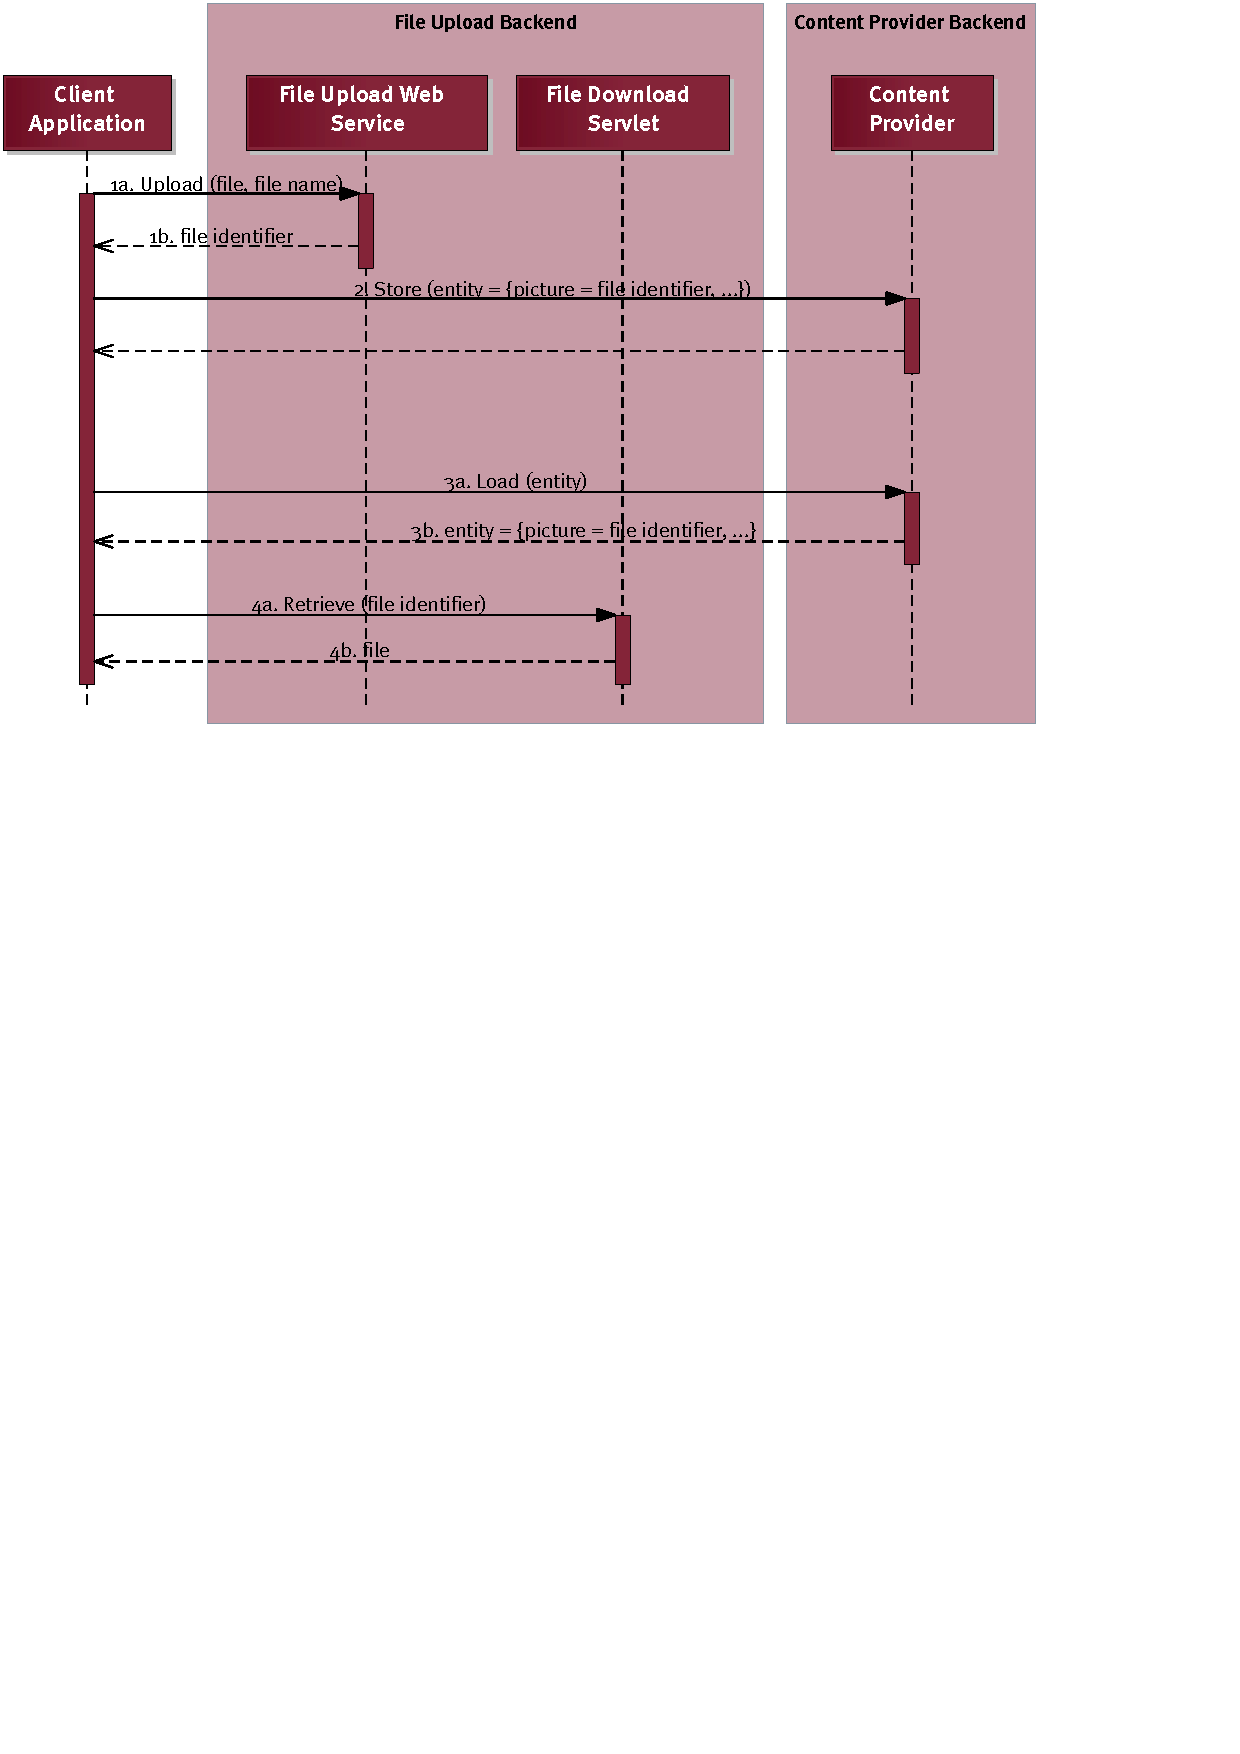
\includegraphics[clip,  trim=0 17.4cm 3.cm 0, scale=0.8]{Fig/upload-sequence.pdf}
\caption{Procedure of uploading and retrieving user-uploaded images}
\label{fig:remoteFileUpload}
\end{figure}

As a further consequence, the uploaded file is not directly stored in the database. Instead, when called by a \lstinline|FileUpload| element, the upload service stores the file on disk at the specified path (\lstinline|storagePath|) and returns an identifier string of this file to the calling client (\Cref{fig:remoteFileUpload}, step 1).
This identifier is then used throughout the model, particularly as the value of a corresponding attribute of type \lstinline|file|  (\Cref{fig:remoteFileUpload}, step 2).

When such an identifier is encountered as the value of an \lstinline|UploadedImageOutput|, this element calls a servlet at the \lstinline|fileUploadConnection|, passing the identifier as a parameter (\Cref{fig:remoteFileUpload}, step 4). That way, the image is downloaded for the client just as soon as it is needed, instead of loading it at every initialisation of entities by a content provider. Note that currently only JPEG images should be uploaded, since the servlet always tries to output any given file using the content type \lstinline|image/jpeg|.



\subsubsection{List of open issues}
\label{sec:listOfOpenIssues}

The \lstinline!md2_list_of_open_issues! comprises all code necessary for displaying the list of open issues within the app. This list shows all workflow instances, whose state is at a workflow element, which belongs to the current app. Currently supported data listed in this widget are the guid of the workflow instance, the workflow element name and the last fired event. 
The list is included as \lstinline!dijit_Widget! and is listed as a \texttt{Tool} within the app.json under the bundle specifications of \lstinline!toolset!. In the \lstinline!ListOfOpenIssuesController! a \lstinline!DataView! is created, which uses the workflow store as a \lstinline!DataViewModel!. The workflow store is described in \cref{workflow_store}.
In addition to just displaying the workflow instances it is possible to start the workflow element through clicking on the respective entry. Therefore the \lstinline!ListOfOpenIssuesController! handles the event \lstinline!onClicked! and calls the function \lstinline!startWorkflow! of the respective \lstinline!MD2MainWidget!. Therefore the workflow instance ID is retrieve in combination with the content provider IDs of its current state. With these the content provider referenced in the \lstinline!workflowStateHandler! are resetted to their respective values.

\subsubsection{Local store} \label{local_store}



The local store within the bundle \lstinline|md2_local_store| is one of three stores used in the context of \mapapps within \MD. This store implements some of the guidelines from the \lstinline|dojo/Store| interface, which means, that it offers the methods \lstinline|query|, \lstinline|get|, \lstinline|put|, \lstinline|add|, and \lstinline|remove|.
The local store can be used by a content provider (set to local within the controller model). This store saves all data as cookies in the browser. Thus the store is not meant for consistent data storage.

\subsubsection{Location service}\todo{@ANDI}
The \lstinline|LocationStoreFactory| provides methods to transfer a longitude and latitude pair into an address (i.e. a country, city, street, postal) and vice versa. In the first case, the method \lstinline|_getAddressForLocation| is used, which takes two parameters for the longitude and latitude value. In the second case, the method \lstinline|_getLocationForAddress| is used. This method takes a single string as input, which contains all the address information (e.g., \textit{Schlossplatz Muenster 48149}). For both methods, the result is a JavaScript "promise" object.

ArcGIS is the underlying API that is used for this (reverse-) geocoding. The URL to use this service is specified in the \lstinline|manifest.json| of that bundle. Currently, the URL is:

 \lstinline|http://geocode.arcgis.com/arcgis/rest/services/World/GeocodeServer|. 

\subsubsection{Runtime}

This bundle contains the main logic of the \MD \mapapps framework, which is mainly based on the \lstinline|MD2MainWidget| object. Most other sub bundles just enhance the functions of this widget.

\paragraph{MD2MainWidget}
The \lstinline!MD2MainWidget! is responsible for the opening, closing, etc. of views. 
Each workflow element (see \ref{sec:developAndDeployMultiApps}) has its own instance of a \MD main widget. This is specified in the respective controller of the workflow element bundle inside the app. That is, the \lstinline!manifest.json! of the workflow element bundle references an \lstinline!_md2AppWidget! for its controller. Once the controller is activated (i.e. the \lstinline!activate! function is called), the respective \MD main widget instance is built. This \MD main widget is implemented in the file \lstinline!MD2MainWidget!, which serves as the basic starting point to start a workflow. Thus, it provides methods to start a workflow element. There are different ways a workflow can be started:
\begin{itemize}
	\item One way is to start it directly from the map.apps tool bar. Each workflow element marked as \lstinline|startable| in the model for this app, gets its own tool. Through clicking on it the method \lstinline|startWorkflowFromTool| is stared, which first resets all current workflow elements and the workflow handlers and then calls the \lstinline|startworkflow| function.
	\item Another way is to start a workflow from the list of open issues (see section \ref{sec:listOfOpenIssues}). Therefore the \lstinline|startWorkflow| is directly started from the \lstinline|OpenIssuesListController|.
\end{itemize}
When the workflow element window is closed and the same operation to start a workflow element is called again (reopening the same entry of the list of open issues or restart the same tool) the same window will all data entered before will be opened. However, when opening another workflow instance in between all changes are dropped!
Each \lstinline|MD2MainWidget| contains a runtime variable \$, which contains important objects needed within the context of the widget. While many objects are created anew for each widget, some objects as the \lstinline|WorkflowStateHandler| (\cref{par:workflowStateHandler}) are globally used and thus only created once. Many of those objects are injected as singletons within the \lstinline|mainfest.json| of the bundle \lstinline|md2_runtime|.
Figure~\ref{fig:InitMD2MainWidget} depicts this initialization process.

\begin{figure}
\centering
\begin{tikzpicture}[
	redbox/.style = {rectangle, fill=ercisred, text =white, draw=none, text centered, drop shadow},
	arrowlbl/.style = {pos=.5, black},
	>=stealth
]

\draw (-3.5,-2.25) rectangle (1.2,-0.5);
\draw [fill=gray!20!white] (-3.5,-0.95) rectangle (-0.7,-0.5) node[pos=.5] {\small{List of open issues}};
\draw [redbox] (-3.3,-2) rectangle (1,-1) node[pos=.5] {OpenIssueListController};

\draw [->, thick, ercisred] (1,-1.1) -- (4.6,-1.1) node[above, arrowlbl] {\lstinline!startWorkflow!} -- (4.6,0.4) -- (6.5,0.4);

\draw [->, thick, ercisred] (1,-1.9) -- node[above, arrowlbl] {\lstinline!getMD2MainWidget!} (6,-1.9);

\node[draw] (tool) at (-1.25, -3) {\small{\textit{map.apps tool}}};
\draw [->, thick, ercisred] (tool) -- (5.35,-3) node[above, arrowlbl] {\lstinline!startWorkflowFromTool!} -- (5.35,0.2) -- (6.5,0.2);

\draw [->, thick, ercisred] (-2.9,1) -- node[above, arrowlbl] {\lstinline!load!} (-1.9,1);

\node [above] at (-0.9,0.5) {\lstinline!activate!};
\draw [->, thick, ercisred] (-1.8,1) -- (-1.8,0.5) -- (0,0.5);
\draw [fill=gray!20!white](-1.9,1.1) rectangle (-0.8,1.5) node[pos=.5] {\small{WfE}};
\draw (-1.9,-0.25) rectangle (2.25,1.5);
\draw [redbox] (0,0) rectangle (2,1) node[pos=.5] {Controller};

\draw [->, thick, ercisred] (2,0.65) -- node[above, arrowlbl] {\lstinline!build!} (6.5,0.65);

\draw [fill=gray!20!white] (5.7,1.1) rectangle (8,1.5) node[pos=.5] {\small{MD2Runtime}};
\draw (5.7,-2.25) rectangle (11.25,1.5);
\draw [redbox] (6.5,0) rectangle (11,1) node[pos=.5] {MD2MainWidget};
%\node [rotate=270] at (10.7,0.35) {\small{startWorkflow}};
%\draw [->, thick, ercisred] (10,0.8) -- (10.5,0.8) -- (10.5,0.2) -- (10,0.2);

\draw [->, thick, ercisred] (7,0) -- node[right, arrowlbl] {\lstinline!register!} (7,-1);

\draw [redbox] (6,-2) rectangle (11,-1) node[pos=.5] {WorkflowStateHandler};

\end{tikzpicture}
\caption{Initialization of the \MD main widget in order to start a workflow}
\label{fig:InitMD2MainWidget}
\end{figure}

\paragraph{Actions}
Each action that is defined in the \MD DSL must also exist in the \MD runtime bundle in map.apps to be used. Individual actions are stored in the subfolder \lstinline!simpleactions!. Moreover, an \lstinline!ActionFactory! must provide a simple method that returns an instance of the respective action (e.g., \lstinline!getLocationAction! for the \lstinline!LocationAction!). All actions provide a method \lstinline!execute! that implements the action. An individual constructor allows to initialize the action, e.g., setting the city's name for a \lstinline!LocationAction!. The \lstinline!ActionFactory! is instanced in the method \lstinline!build! of the \lstinline!MD2MainWidget! (see figure~\ref{fig:InitMD2MainWidget}). Thus, every workflow element can access and use this factory.

\paragraph{Content Provider}
The content providers are responsible for saving and persisting the state of one or many objects. While the generated code just provides factories for the creation of content providers the actual code is positioned within the static bundles. Each content provider is instantiated with an unique name, the app ID it belongs to, a store (either remote or local), the information if it is a provider for a list of objects, a filter restricting the queried items and the information if it is a remote or a local store.
Besides functions to get or set the content of the provider, functions are offered to access the injected store and persist the data.
Additionally each content provider can inform other components of the app about changes within attributes. This can be used for example to refresh the values of view elements.
The function \lstinline|restore| and \lstinline|reset| are used within the \lstinline|WorkflowStateHandler| to be able to influence the state of the content provider, when the workflow instance is changed.

\paragraph{Data Mapper}
Whenever a value within a content provider changes it is necessary to inform the view elements to be able to refresh them. This is one within the classes of this folder.

\paragraph{Data Types}
In this folder all data types known by the \MD \mapapps framework are listed. Each data type provides additional functions for working with the data objects such as cast or compare operations. The \lstinline|TypeFactory| is used to instantiate an object according to its data type and is injected to the runtime variable \$ within the \lstinline|MD2MainWidget|.

\paragraph{Entities}
This folder contains all internal entities known to the \MD \mapapps framework. This is the \lstinline|Location| entity and the abstract class \lstinline|_Entity|, which is inherited by all generated entities.

\paragraph{Events}
In the \MD modelling language it is possible to define actions based on events. Examples for such events are changes or clicks on view elements. To be able to map this behaviour in \mapapps each possible events has its own class, which subscribes a topic associated with the type of event it represents. The \lstinline|EventRegistry| has a list of all possible events and the root event classes enable to register actions to the specific events.

\paragraph{Handler}
This folder contains handlers form global events. This mainly results in info or warning messages being displayed. Therefore certain actions are bound to events by subscribing to topics. One example is the data action bound to the topic \lstinline[language=Javascript]|"md2/contentProvider/dataAction/${appId}"|. If any component is publishing a status (\lstinline[language=Javascript]|"success"| or \lstinline[language=Javascript]|"error"|) for an action (e.g. \lstinline[language=Javascript]|"load"| or \lstinline[language=Javascript]|"save"|) a respective info message is shown in the lower right corner of the website.

\paragraph{Resources}
This folder contains images and style files.

\paragraph{Templates}
This folder contains the root html file of the \lstinline|MD2MainWidget|.

\paragraph{Validators}
In the model validators can be defined for view elements. This folder contains all existing validators, which can be created using the \lstinline|ValidatorFactory| which is injected in the runtime variable \$.

\paragraph{View}
The \lstinline|MD2MainWidget| is responsible for creating the views for the workflow elements. For this purpose it uses a \lstinline|ViewManager| which creates the view elements based on the \lstinline|view| entries within the manifest.json of the respective workflow element. The type of a view element is therefore linked to a dataform component either contained in the bundle \lstinline|md2_formcontrols| or within the external conterra bundle \lstinline|base/dataform|.

\paragraph{Workflow}\label{par:workflowStateHandler}
The \lstinline|WorkflowStateHandler| together with the generated \lstinline|WorkflowEventHandler| are responsible for managing the state of the current workflow instance. This includes the transitions between workflow elements within the context of one and as well as firing workflow events to the backend.  
For each started workflow instance an unique ID is generated and assigned to that instance. This is done in the method \lstinline!startWorfklow! of the \lstinline!MD2MainWidget!. A \lstinline!WorkflowStateHandler! provides methods to set and get the currently active workflow instance ID in a global context. This information is needed to suspend a workflow and to resume that workflow at a later time. The variable \lstinline|_lastStartedTool| provides information about how the workflow instance has been started. This is important when it comes to decide for a new \lstinline!startWorfklow! evaluation, if the current workflow instance has to be resumed or a new one should be created.

To change the current workflow element, the \lstinline|WorkflowStateHandler| provides to methods \lstinline|changeWorkflowElement| and \lstinline|fireEventToBackend|. 
The first one  just opens another \lstinline|MD2MainWidget|, since the workflow is continued in the same app.
The later one, on the other hand, will exit the workflow instance for the current app and close all windows, since the workflow is supposed to continue in another app. Additionally the backend is informed about this step by eventually calling the \lstinline|fireEventToBackend| of the \lstinline|WorkflowStore| (\cref{workflow_store}). Since the \lstinline|WorkflowStore| is supposed to send the content provider ids, this leads to a problem. 
The saving operation of the content providers is usually done shortly before the workflow event is fired. Since the content provider ids are not set until the backend has answered to the webservice calls, they may not be accessible already. For this purpose the \lstinline|WorkflowStateTransaction| is used. 
With a new workflow instance id a new transaction is created as well. It keeps a list of all started content provider saving operations and allows only to fire a workflow event, when no operation is in progress. Additionally the transaction is informed via a subscription about each termination of a content provider operation and will then retry to fire a workflow element, if one was queued before.

\subsubsection{Store}\label{store}

The \lstinline|md2_store| bundle provides the second of the three stores. It could also be called remote store, since it provides access to external data storage. It is again an implementation of the \lstinline|dojo/Store| through implementing the necessary functions. The store is used within a content provider to query the current state of the objects belonging to the current workflow instance. In contrast to the local store, data which is saved within this store is persisted throughout the whole application landscape. For this purpose each store needs to be provided with an url, pointing to the respective backend server. The data is then queried and stored using rest web services. One implementation of such a backend is automatically generated by the backend generator described in \cref{sec:backend}. For the store to be able to find its respective backend the urls need to match each other (see \cref{subsubsec:Backend}). 

\subsubsection{Workflow Store} \label{workflow_store}

The workflow store within \lstinline|md2_workflow_store| differs from the other stores provided by the static bundles. While the local (\cref{local_store} the remote store (\cref{store}) are used within a content provider the workflow store has its own purposes. This store is used to save and query the status of all workflow instances. On the one side it is injected in the \lstinline|WorkflowStateTransaction| of the \lstinline|md2_runtime| bundle (see \cref{par:workflowStateHandler}). There it is responsible of informing the backend of an change within the workflow instance. In the model this action can be represented by the \lstinline|FireEventAction|. Beside the information which event has been fired and which was the current workflow element and instance id, the backend get a list of all ids registered in the content providers. This is necessary to be able to restore the state of the content providers in another app.

On the other hand the workflow store is referenced in the list of open issues. The workflow store implements, same as the other, the functions of the \lstinline|dojo/Store|. Through this it is possible to hand the workflow store over to a \lstinline|DataView|, which then displays the information retrieved from the store. While the \lstinline|query| function enables to query the whole list of the list of open issues

For the workflow store to work, the app.json needs to provide appropriate configuration for the REST location and the current app ID, for which the web service should filter. The following snippet (with equivalent values) is automatically generated:
\begin{lstlisting}[language=Javascript]
"md2_workflow_store": {
	"MD2WorkflowStore": {
		"uri": "http://localhost:8080/ReferenceProject.backend/service/workflowState/",
		"app": "Citizenapp"
	}
}
\end{lstlisting}

% end of section for static map.apps implementation

\subsection{Generated map.apps implementation} \todo{Maybe join this with the \enquote{map.apps Generator} section}



\section{Backend}\label{sec:backend}\todo{Das hier in extra .tex Datei auslagern, weil jetzt extra section??}

The \MD backend is implemented in Java. It is generated by the \MD framework from the \MD model. Some code in the backend is static, though. 

\subsection{Beans}
\label{subsec:beans}
For entities that are used in at least one remote content provider a stateless session bean is generated. Such a bean provides basic methods to create or manipulate entities of that bean. JPA is used for the persistent storage of the data. The persistence configuration file is located at \lstinline|META-INF/persistence.xml|. Currently, EclipseLink as persistence service.

Additionally, a static session bean is generated for the workflow state of the instances of a workflow. Internally, a workflow instance is identified by an identification number that is represented as an integer. However, since a workflow instance is generated at the client side, a single client cannot assure that a specific number is not used by another workflow instance of another client. Therefore, every client generates its own \lstinline|instanceId| that is a hash value of the current time (among others), and thus a quite likely unique identification value. This generated hash value is represented as a string value.

\subsection{Datatypes}
The datatypes used in the backend are static and implemented as simple wrappers. For instance, every entity has a unique internal identification number (\lstinline|internalID|) that is an integer value. The respective wrapper implementation is depicted in the following listing. 

\begin{lstlisting}[language=Java, label=lst:intIdWrapper, caption=An integer wrapper for the internal identification number]
@XmlRootElement(name = "internalId")
public class InternalIdWrapper {
	
	@XmlElement
	protected int __internalId;
	
	protected InternalIdWrapper() {
		// no-arg default constructor necessary
	}
	
	public InternalIdWrapper(int integer) {
		this.__internalId = integer;
	}
}
\end{lstlisting}

\subsection{Entities}
The entities and enumerations defined in the \MD model are generated into the subpackage \lstinline|entities.models|. Moreover, two static Java classes are generated:  \lstinline|RequestDTO| and \lstinline|WorkflowState|. The former is used as an encapsulation for all client requests, e.g., to create a corresponding REST request. The latter is used as a representation of the state an instance of a workflow has. A workflow can consist of multiple workflow elements, that in turn can fire different events. Thus, every started workflow (i.e. every workflow instance) must keep track of its current workflow element and the last fired event in it.

\subsection{Filedownload}\todo{Please give me a description... @JAN}

\subsection{Webservices}
Similar to the generation of the stateless session beans, a webservice is only generated for those entities that are used in at least one remote content provider. Those webservice provide a simple access to the entity data.

Additionally, some static webservice are generated that are used for specific features. Those webservices are explained in the following.
\subsubsection{Call external websevice}
As a simple way to interact with external services, a webservice \lstinline|CallExternalWebServiceWS| in the backend allows to call another webservice, that might be on a different system or server. The webservice in the backend provides a method that takes a JSON-encoded object as an input. This object must contain the URL, the REST method type and the set of parameters of that method. For example, the following listing depicts how such a JSON object is constructed in map.apps.

\begin{lstlisting}[language=Javascript, label=lst:callExtWSJSON, caption=JSON-encoded object containing information to call an external webservice]
data: json.stringify({
  "url": this._url,
  "requestMethod": this._method,
  "queryParams": this._queryParams,
  "body": this._bodyParams
})
\end{lstlisting}

\subsubsection{Event handler} 

For the communication across apps, the backend offers an event handler webservice. This webservice handles all workflow events that are fired in one app and start a workflow element in another app, i.e. it is necessary for all switches between apps. Required parameters for this webservice are

\begin{itemize}
\item the instance ID of the workflow instance,
\item the event which was fired,
\item the content provider IDs,
\item and the current workflow element which fired the event.
\end{itemize}

The event handler webservice uses these parameters to perform adjustments in the workflow state of the current workflow instance. This includes setting the last event fired and the current workflow element. Furthermore, the content provider IDs are stored in the workflow state so that subsequent apps can load data from content providers using these IDs.

\subsubsection{Workflow state} 

The workflow state webservice allows to retrieve open workflow instances or add new ones. Whenever the list of open issues is opened in an app, this app sends its name to the workflow state webservice. The webservice then returns all workflow states whose current workflow element is part of the app with the given app name. For this purpose, the belongingness of workflow elements to apps is originally derived from the DSL model and stored in a hashmap in the backend.

Furthermore, for every new workflow instance, a new workflow state needs to be created. To do so, the workflow state webservice is called as soon as the app which started the workflow hands the control over to the backend. This app generates a globally unique if as described in \ref{subsec:beans} and provides it in the webservice call.

\subsubsection{File upload} \todo{@JAN Please give me a description...}

\subsubsection{Version negotiation} \todo{Please give me a description...}


